\documentclass[11pt,letterpaper]{article}
\usepackage[lmargin=1in,rmargin=1in,tmargin=1in,bmargin=1in]{geometry}
\usepackage{../style/homework}
\usepackage{../style/commands}
\setbool{quotetype}{false} % True: Side; False: Under
\setbool{hideans}{false} % Student: True; Instructor: False

% -------------------
% Content
% -------------------
\begin{document}

\homework{5: Due 06/01}{Science, my lad, is made up of mistakes, but they are mistakes which it is useful to make, because they lead little by little to the truth.}{Jules Verne}

% Problem 1
\problem{10} Define what makes a function linear. What `form' does every linear function of one-variable have? \pspace

\sol A linear function is a function which has a constant rate of change. Therefore, `anything' with a constant rate of change is a linear function. In one variable, every linear function has the form $y= mx + b$ for some $m$ and $b$. 



\newpage



% Problem 2
\problem{10} Being as accurate as possible, sketch the graph of the line $-3x + 5y= 10$.
	\[
	\fbox{
	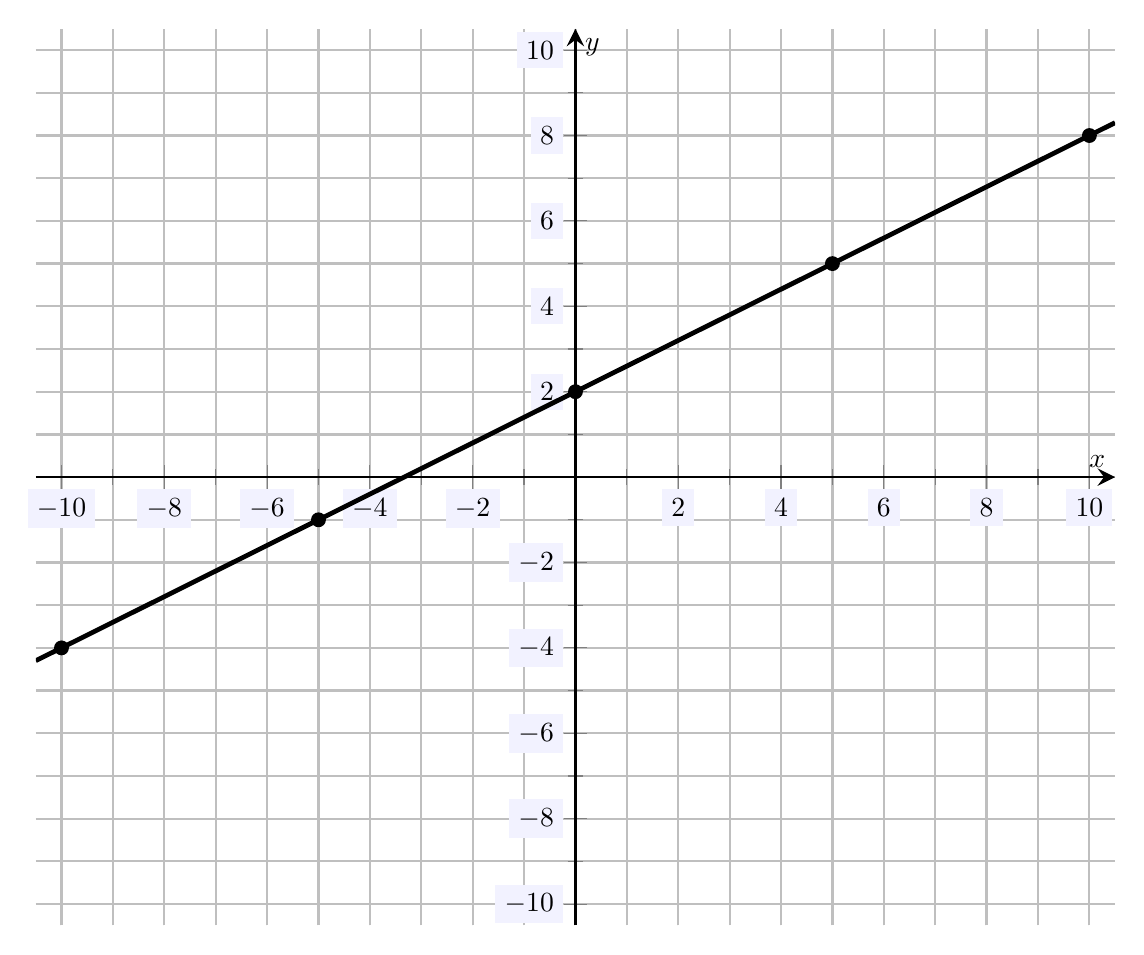
\begin{tikzpicture}[scale=2,every node/.style={scale=0.5}]
	\begin{axis}[
	grid=both,
	axis lines=middle,
	ticklabel style={fill=blue!5!white},
	xmin= -10.5, xmax=10.5,
	ymin= -10.5, ymax=10.5,
	xtick={-10,-8,-6,-4,-2,0,2,4,6,8,10},
	ytick={-10,-8,-6,-4,-2,0,2,4,6,8,10},
	minor tick = {-10,-9,...,10},
	xlabel=\(x\),ylabel=\(y\),
	]
	\addplot[black, line width=0.03cm, domain=-10.5:10.5] ({x},{3/5*x+2});
	\draw[fill=black] (-10,-4) circle (0.04cm);
	\draw[fill=black] (-5,-1) circle (0.04cm);
	\draw[fill=black] (0,2) circle (0.04cm);
	\draw[fill=black] (5,5) circle (0.04cm);
	\draw[fill=black] (10,8) circle (0.04cm);
	\end{axis}
	\end{tikzpicture}
	}
	\] \pspace

\sol We have\dots \pspace
	\[
	\begin{aligned}
	-3x + 5y&= 10 \\
	5y&= 3x + 10 \\
	y&= \tfrac{3}{5}\,x + 2
	\end{aligned}
	\] \pspace
Therefore, this is a line with slope $\tfrac{3}{5}$ and $y$-intercept $(0, 2)$. Using the fact that $m= \tfrac{3}{5}$ and recalling that $m= \dfrac{\Delta y}{\Delta x}$, we can interpret the slope as for every 5 increase in $x$, there is a corresponding increase of 3 in $y$. Equivalently, writing the slope as $m= \tfrac{3}{5}= \tfrac{-3}{-5}$, we can see that for every decrease of 5 in $x$ results in a corresponding decrease of 3 in $y$. Starting at the $y$-intercept $(0, 2)$, we can then sketch out the line using these interpretations. 



\newpage



% Problem 3
\problem{10} Determine if the following function is linear. Explain why or why not.
	\begin{table}[!ht]
	\centering
	\begin{tabular}{c|c}
	$x$ & $f(x)$ \\ \hline
	$0.5$ & $26.45$ \\
	$1.8$ & $21.64$ \\
	$3.9$ & $13.87$ \\
	$4.2$ & $13.44$ \\
	$5.5$ & $7.95$ \\
	$8.1$ & $-1.67$
	\end{tabular}
	\end{table} \pspace

\sol A linear function has a constant rate of change, e.g. a constant slope. We can take two points at a time to compute the slopes: \pspace
	\[
	\begin{aligned}
	m&= \dfrac{\Delta y}{\Delta x}&= \dfrac{21.64 - 26.45}{1.8 - 0.5}= \dfrac{-4.81}{1.3}= -3.7 \\[0.3cm]
	m&= \dfrac{\Delta y}{\Delta x}&= \dfrac{13.87 - 21.64}{3.9 - 1.8}= \dfrac{-7.77}{2.1}= -3.7 \\[0.3cm]
	m&= \dfrac{\Delta y}{\Delta x}&= \dfrac{13.44 - 13.87}{4.2 - 3.9}= \dfrac{-0.43}{0.3}= -1.433 \\[0.3cm]
	m&= \dfrac{\Delta y}{\Delta x}&= \dfrac{7.95 - 13.44}{5.5 - 4.2}= \dfrac{-5.49}{1.3}= -4.223 \\[0.3cm]
	m&= \dfrac{\Delta y}{\Delta x}&= \dfrac{-1.67 - 7.95}{8.1 - 5.5}= \dfrac{-9.62}{2.6}= -3.7
	\end{aligned}
	\] \pspace
Because the slope is not constant, the data for the function in the table above cannot represent a linear function. 



\newpage



% Problem 4
\problem{10} Consider the linear equation $15x + 3y= 39$. 
        \begin{enumerate}[(a)]
        \item Solve the linear equation for $y$. 
        \item Determine the slope and $y$-intercept for the corresponding line.
        \item Interpret the slope in at least two different ways. 
        \end{enumerate} \pspace

\sol
\begin{enumerate}[(a)]
\item We have\dots \pspace
	\[
	\begin{aligned}
	15x + 3y= 39 \\[0.3cm]
	3y= -15x + 39 \\[0.3cm]
	y= -5x + 13
	\end{aligned}
	\] \pspace

\item Because $y= -5x + 13$ is of the form $y= mx + b$ with $m= -5$ and $b= 13$, the slope is $-5$ and the $y$-intercept is 13, i.e. $(0, 13)$. \pspace

\item We have $m= -5= \dfrac{-5}{1}$. Because $m= \dfrac{\Delta y}{\Delta x}$, we can interpret this as $\Delta x= 1$ and $\Delta y= -5$, i.e. every increase by 1 in $x$ results in a decrease in $y$ by 5. Equivalently, using the fact that $m= -5= \dfrac{5}{-1}$ and $m= \dfrac{\Delta y}{\Delta x}$, we can interpret this as $\Delta x= -1$ and $\Delta y= 5$, i.e. every decrease by 1 in $x$ results in an increase in $y$ by 5.
\end{enumerate}



\newpage



% Problem 5
\problem{10} Consider the line given by $y= \frac{11}{4}\,x - 6$.
        \begin{enumerate}[(a)]
        \item Put the line in standard form.
        \item Is the point $(-12, -27)$ on the line? Explain.
        \item Is the point $(8, 16)$ on the line? Explain. 
        \end{enumerate} \pspace

\sol
\begin{enumerate}[(a)]
\item We have\dots
	\[
	\begin{aligned}
	y= \dfrac{11}{4}\,x - 6 \\
	4y= 4 \left( \dfrac{11}{4}\,x - 6 \right) \\
	4y= 11x - 24 \\
	-11x + 4y= -24
	\end{aligned}
	\] 

\item If the point $(-12, -27)$ is on the line, then when $x= -12$ we know that $y= -27$. But we have\dots
	\[
	y(-12)= \dfrac{11}{4} \cdot -12 - 6= 11 \cdot -3 - 6= -33 - 6= -39
	\]
Therefore, the point $(-12, -27)$ is not on the line. However, the point $(-12, -39)$ is on the line. Equivalently, the point $(-12, -27)$ is on the line if it satisfies the equation $-11x + 4y= -24$. We have\dots
	\[
	\begin{aligned}
	-11x + 4y&= -24 \\
	-11(-12) + 4(-27)&\stackrel{?}{=} -24 \\
	132 - 108&\stackrel{?}{=} -24 \\
	24&\neq -24 \\
	&\text{ \xmark}
	\end{aligned}
	\]

\item If the point $(8, 16)$ is on the line, then when $x= 8$ we know that $y= 16$. But we have\dots
	\[
	y(8)= \dfrac{11}{4} \cdot 8 - 6= 11 \cdot 2 - 6= 22 - 6= 16
	\]
Therefore, the point $(8, 16)$ is on the line. Equivalently, the point $(8, 16)$ is on the line if it satisfies the equation $-11x + 4y= -24$. We have\dots
	\[
	\begin{aligned}
	-11x + 4y&= -24 \\
	-11(8) + 4(16)&\stackrel{?}{=} -24 \\
	-88 + 64&\stackrel{?}{=} -24 \\
	-24&\neq -24 \\
	&\text{ \cmark}
	\end{aligned}
	\] 
\end{enumerate}



\newpage



% Problem 6
\problem{10} A linear function has a table whose values are given below. Find the equation of the linear function. Be sure to specify the slope and $y$-intercept.
	\begin{table}[!ht]
	\centering
	\begin{tabular}{c|c}
	$x$ & $f(x)$ \\ \hline
	$3$ & $5.7$ \\ 
	$4$ & $2.4$ \\
	$7$ & $-7.5$ \\
	$11$ & $-20.7$
	\end{tabular}
	\end{table} \pspace

\sol We have\dots \pspace
	\[
	\begin{aligned}
	m&= \dfrac{2.4 - 5.7}{4 - 3}= \dfrac{-3.3}{1}= -3.3 \\[0.3cm]
	m&= \dfrac{-7.5 - 2.4}{7 - 4}= \dfrac{-9.9}{3}= -3.3 \\[0.3cm]
	m&= \dfrac{-20.7 - (-7.5)}{11 - 7}= \dfrac{-13.2}{4}= -3.3
	\end{aligned}
	\] \pspace
Because the slope is constant, we know that the function given by the table of values above is linear. Because the function is clearly not vertical, we know that it is of the form $f(x)= mx + b$. By the work above, we know that $m= -3.3$ so that $y= -3.3x + b$. However, the function also contains the point $(3, 5.7)$ so that\dots \pspace
	\[
	\begin{aligned}
	f(x)= -3.3x + b \\[0.3cm]
	5.7= -3.3(3) + b \\[0.3cm]
	5.7= -9.9 + b \\[0.3cm]
	b= 15.6
	\end{aligned}
	\] \pspace
Therefore, the function is $f(x)= -3.3x + 15.6$. Because $f(x)$ is of the form $y= mx + b$ with $m= -3.3$ and $b= 15.6$, we know that the slope is $-3.3$ and the $y$-intercept is 15.6, i.e. $(0, 15.6)$. 



\newpage



% Problem 7
\problem{10} Consider the linear function $f(x)= \dfrac{4 - 3x}{2}$.
	\begin{enumerate}[(a)]
	\item Find the slope of this linear function. 
	\item Interpret the slope two different ways.
	\item Is the linear function increasing, decreasing, or constant? Explain. 
	\item Determine the $y$-intercept for $f(x)$.
	\item Determine the $x$-intercept for $f(x)$.
	\end{enumerate} \pspace

\sol
\begin{enumerate}[(a)]
\item We have $f(x)= \dfrac{4 - 3x}{2}= 2 - \frac{3}{2}\,x$ so that the slope is $m= -\frac{3}{2}$. 

\item We have $m= -\dfrac{3}{2}= \dfrac{-3}{2}$. Because $m= \dfrac{\Delta y}{\Delta x}$, we can interpret this as $\Delta x= 2$ and $\Delta y= -3$, i.e. every increase by 2 in $x$ results in a decrease in $y$ by 3. Equivalently, using the fact that $m= -\dfrac{3}{2}= \dfrac{3}{-2}$ and $m= \dfrac{\Delta y}{\Delta x}$, we can interpret this as $\Delta x= -2$ and $\Delta y= 3$, i.e. every decrease by 2 in $x$ results in an increase in $y$ by 3. Finally, we can also use the fact that $m= -\dfrac{3}{2}= -1.5$ so interpret the slope as every increase of 1 in $x$ results in a decrease of 1.5 in $y$, or that every decrease of 1 in $x$ results in an increase of 1.5 in $y$. 

\item Because $m= -\frac{3}{2} < 0$, we know that $f(x)$ is a decreasing function. 

\item We have $f(x)= \dfrac{4 - 3x}{2}= -\frac{3}{2}\,x + 2$, which is in the form $y= mx + b$. Therefore, the $y$-intercept is 2, i.e. $(0,\, 2)$. Equivalently, the $y$-intercept occurs when $x= 0$. But then $f(0)= \dfrac{4 - 3(0)}{2}= \dfrac{4}{2}= 2$ is the $y$-intercept, i.e. the point $(0,\, 2)$. 

\item The $x$-intercept occurs when $f(x)= 0$. But then we have\dots
	\[
	\begin{aligned}
	f(x)&= \dfrac{4 - 3x}{2} \\[0.3cm]
	0&= \dfrac{4 - 3x}{2} \\[0.3cm]
	2 \cdot 0&= 2 \cdot \dfrac{4 - 3x}{2} \\[0.3cm]
	0&= 4 - 3x \\[0.3cm]
	3x&= 4 \\[0.3cm]
	x&= \dfrac{4}{3}
	\end{aligned}
	\]
Therefore, the $x$-intercept is $\frac{4}{3}$, i.e. the point $(\frac{4}{3},\,  0)$. 
\end{enumerate} 



\newpage



% Problem 8
\problem{10} You are driving back to college after summer break. It is 12~pm and you are traveling on the highway at a constant speed of 65~mph. Currently, you are 211~mi from college. Let $D(t)$ denote your distance, in miles, that you are from the college $t$ hours from now. 
	\begin{enumerate}[(a)]
	\item Explain why $D(t)$ is linear.
	\item Find $D(t)$. 
	\item What do the slope and $y$-intercept of $W(t)$ represent in context?
	\item Determine when you will arrive at the college. 
	\end{enumerate} \pspace

\sol
\begin{enumerate}[(a)]
\item Because the car is traveling at a constant rate of 65~mph, the distance you have driven towards the college is increasing at a constant rate. But then the distance between you and the college, $D(t)$, is decreasing at a constant rate. Therefore, $D(t)$ is a linear function of $t$.

\item Let $t$ be the number of hours from 12~pm. We know that $D(t)$ is linear so that it has the form $D(t)= mt + b$. Because you are traveling towards the college at a constant rate of 65~mph, the distance, $D(t)$, between you and the college is decreasing at a rate of 65~miles every hour. But then we know that $m= -65$ so that $D(t)= -65t + b$. We know that now, i.e. $t= 0$, you are 211~mi from the college, i.e. the point $(0, 211)$ is on the graph of $D(t)$. But then\dots
	\[
	\begin{aligned}
	D(t)&= -65t + b \\[0.3cm]
	211&= -65(0) + b \\[0.3cm]
	211&= 0 + b \\[0.3cm]
	b&= 211
	\end{aligned}
	\]
Therefore, $D(t)= -65t + b$. Equivalently, because $D(t)= -65t + b$ has $y$-intercept 211, i.e. $(0, 211)$, we know that $b= 211$. 

\item The slope $m= -65$ is the rate of change of the distance between you and the college, i.e. the speed the car is traveling. Every hour, the distance between you and the college decreases by 65~mi. The $y$-intercept is $(0, 211)$, i.e. 211~mi. This represents the initial distance between you and the college, i.e. how far you are from the college at 12~pm. 

\item When you have arrived at the college, the distance between you and the college is 0~mi, i.e. $D(t)= 0$. But then\dots
	\[
	\begin{aligned}
	D(t)&= 0 \\[0.3cm]
	-65t + 211&= 0 \\[0.3cm]
	-65t&= -211 \\[0.3cm]
	t&= \dfrac{211}{65} \\[0.3cm]
	t&\approx 3.246
	\end{aligned}
	\]
Therefore, you will arrive at the college in another 3.246~hours, i.e. 3~hours, 14~minutes, and 46~seconds. At this constant rate, you will arrive at the college at 3:14~pm. 
\end{enumerate}



\newpage



% Problem 9
\problem{10} Showing all your work, find the equation of the line with slope $-\frac{1}{3}$ that passes through the point $(9, 4)$. \pspace

\sol Because the line is not vertical, it must have the form $y= mx + b$. The slope is $-\frac{1}{3}$ so that $y= -\frac{1}{3}\,x + b$. But the line contains the point $(9, 4)$ so that
	\[
	\begin{aligned}
	y&= -\dfrac{1}{3}\, x + b \\[0.3cm]
	4&= -\dfrac{1}{3} \cdot 9 + b \\[0.3cm]
	4&= -3 + b \\[0.3cm]
	b&= 7
	\end{aligned}
	\]
Therefore, $y= -\dfrac{1}{3}\,x + 7$. 



\newpage



% Problem 10
\problem{10} Showing all your work, find the equation of the line that has $x$-intercept $(-2, 0)$ and $y$-intercept $(0, -5)$. \pspace

\sol Because the line is clearly not vertical, we know that the line has the form $y= mx + b$. The line contains the points $(-2, 0)$ and $(0, -5)$ so that\dots \pspace
	\[
	\begin{aligned}
	m= \dfrac{0 - (-5)}{-2 - 0}= \dfrac{0 + 5}{-2 - 0}= \dfrac{5}{-2}= -\dfrac{5}{2}
	\end{aligned}
	\] \pspace
Then $y= -\frac{5}{2}\,x + b$. But the line also contains the point $(0, -5)$, so that
	\[
	\begin{aligned}
	y&= -\dfrac{5}{2}\, x + b \\[0.3cm]
	-5&= -\dfrac{5}{2} \cdot 0 + b \\[0.3cm]
	-5&= 0 + b \\[0.3cm]
	b&= -5
	\end{aligned}
	\]
Therefore, $y= -\dfrac{5}{2}\,x - 5$. 


\end{document}